\section{Results}
Results for two different cases are being presented, one the one-dimensional Ising Model and another for the the two-dimensional Ising model. We begin with looking at the. 1D Ising model.

\subsection{1D Ising model}
\subsubsection{Fitting with linear regression}
For linear regression we got coefficients of $\bm{J}$ in \eqref{eq:1d-ising-linreg} as the following presented in figure \ref{fig:bias-var-franke},
\begin{figure}[H]
    \centering
    \begin{subfigure}[b]{0.9\textwidth}
        \includegraphics[trim={1.5cm 3.5cm 0 3.5cm},clip, scale=1]{../fig/{regression_ising_1d_heatmap_lambda0.001}.pdf}
        \caption{$\lambda=10^{-3}$}
        \label{fig:linreg-hm-1e-3}
    \end{subfigure} \\
    \begin{subfigure}[b]{0.9\textwidth}
        \includegraphics[trim={1.5cm 3.5cm 0 3.5cm},clip, scale=1]{../fig/{regression_ising_1d_heatmap_lambda0.1}.pdf}
        \caption{$\lambda=10^{-1}$}
        \label{fig:linreg-hm-1e-1}
    \end{subfigure} \\
    \begin{subfigure}[b]{0.9\textwidth}
        \includegraphics[trim={1.5cm 3.5cm 0 3.5cm},clip, scale=1]{../fig/{regression_ising_1d_heatmap_lambda10.0}.pdf}
    \caption{$\lambda=10^{1}$}
        \label{fig:linreg-hm-1e2}
    \end{subfigure}
    \caption{Heat map plots of the $\bm{J}$ in \eqref{eq:1d-ising-linreg} retrieved from OLS, Ridge and Lasso. Gathered using $N_\mathrm{train}=5000$.}
    \label{fig:bias-var-franke}
\end{figure}

The $R^2$ score of the OLS, Ridge and Lasso can be seen in figure \ref{fig:linreg-r2},
\begin{figure}[H]
    \centering
    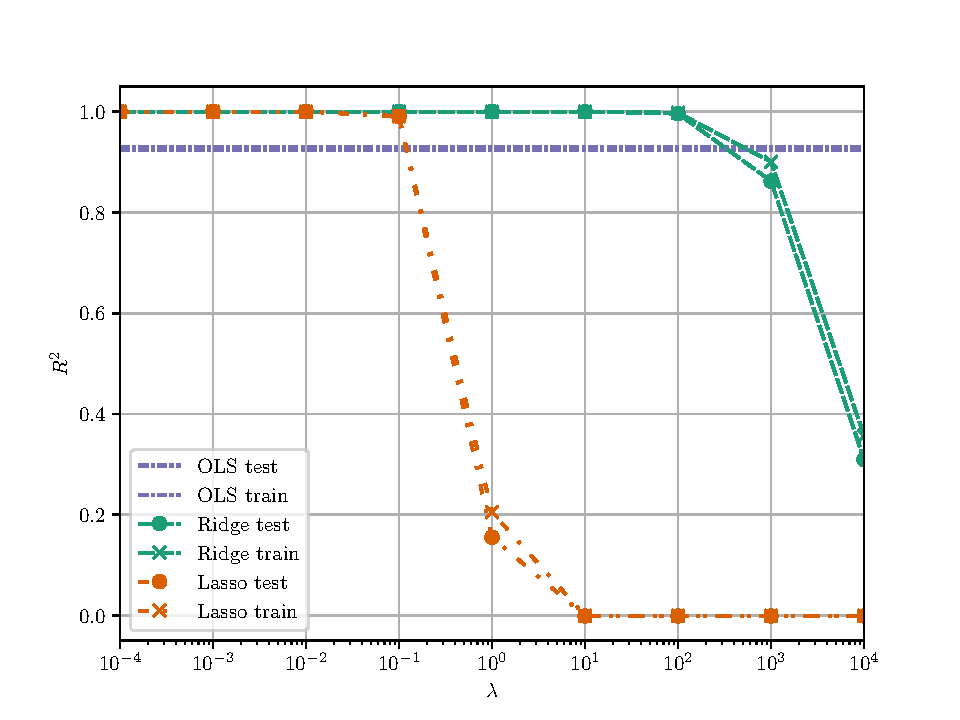
\includegraphics[scale=1.0]{../fig/r2_ols_ridge_lasso.pdf}
    \caption{$R^2$ score for different Ordinary Least Squares(OLS), Ridge and Lasso regression. Retrieved $N_\mathrm{train}=5000$ on a 1D Ising model of size $L=20$.}
    \label{fig:linreg-r2}
\end{figure}

The bias-variance decomposition for Ridge and Lasso using bootstrap and cross validation can be viewed in figure \ref{fig:linreg-bias-variance-decomp-ridge} and \ref{fig:linreg-bias-variance-decomp-lasso}.

\begin{figure}[H]
    \centering
    \begin{subfigure}[b]{0.5\textwidth}
        \centering
        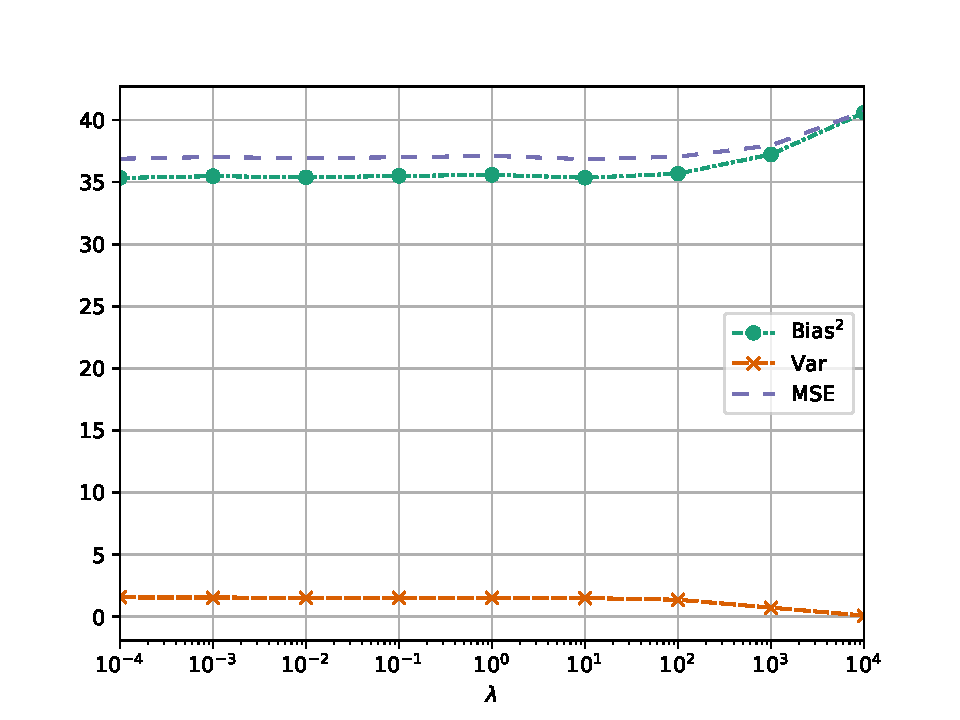
\includegraphics[scale=0.5]{../fig/ridge_bs_bias_variance_analysis.pdf}
        \caption{Bootstrap.}
        \label{fig:linreg-bias-variance-decomp-bs-ridge}
    \end{subfigure}%
    \begin{subfigure}[b]{0.5\textwidth}
        \centering
        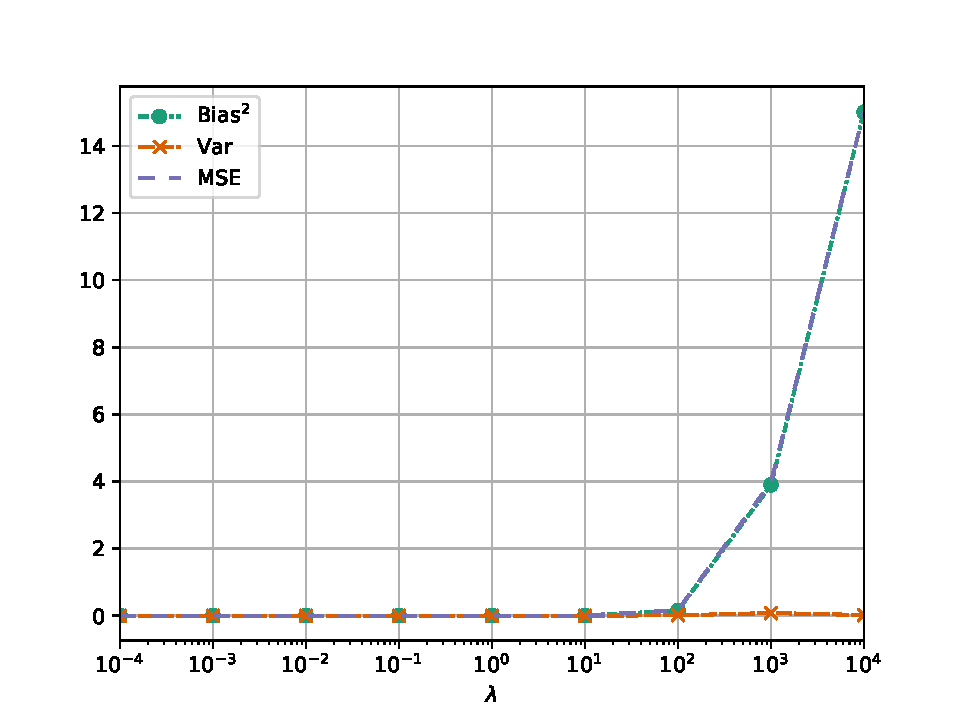
\includegraphics[scale=0.5]{../fig/ridge_cv_bias_variance_analysis.pdf}
        \caption{$k$-fold Cross Validation.}
        \label{fig:linreg-bias-variance-decomp-cv-ridge}
    \end{subfigure}
    \caption{A bias-variance decomposition of Ridge regression using bootstrapping\ref{fig:linreg-bias-variance-decomp-bs-ridge} and cross-validation\ref{fig:linreg-bias-variance-decomp-cv-ridge}.}
    \label{fig:linreg-bias-variance-decomp-ridge}
\end{figure}

\begin{figure}[H]
    \centering
    \begin{subfigure}[b]{0.5\textwidth}
        \centering
        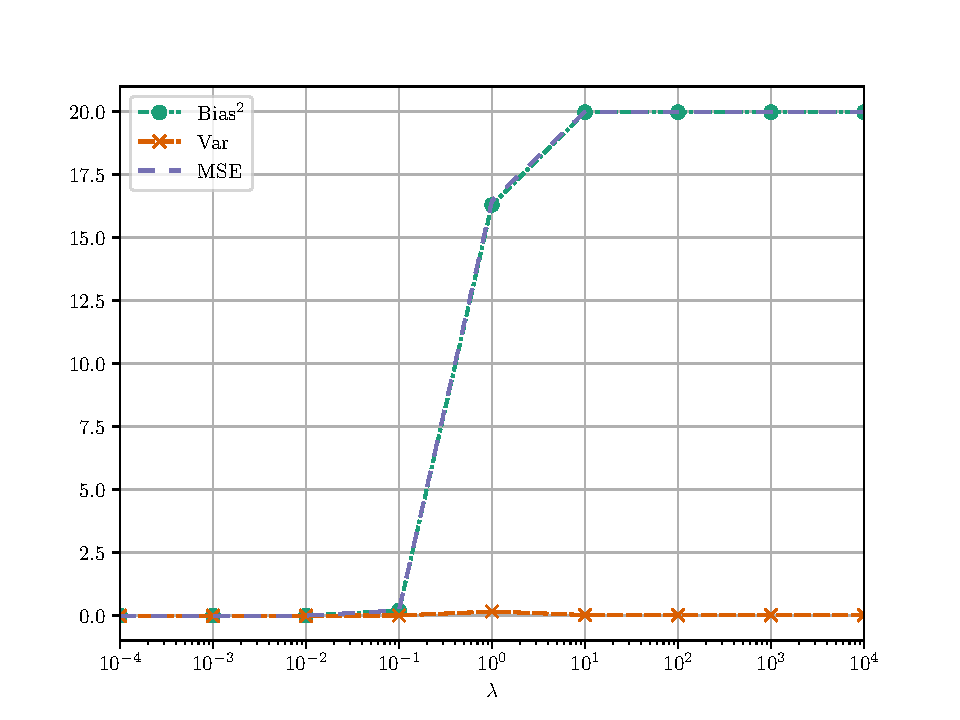
\includegraphics[scale=0.5]{../fig/lasso_bs_bias_variance_analysis.pdf}
        \caption{Bootstrap.}
        \label{fig:linreg-bias-variance-decomp-bs-lasso}
    \end{subfigure}%
    \begin{subfigure}[b]{0.5\textwidth}
        \centering
        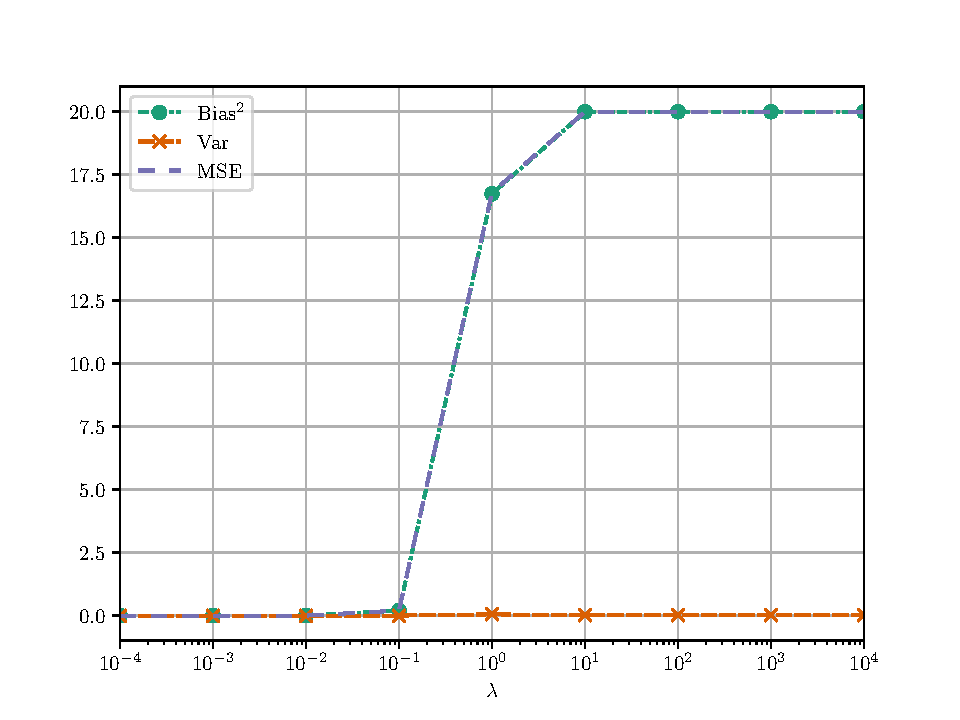
\includegraphics[scale=0.5]{../fig/lasso_cv_bias_variance_analysis.pdf}
        \caption{$k$-fold Cross Validation.}
        \label{fig:linreg-bias-variance-decomp-cv-lasso}
    \end{subfigure}
    \caption{A bias-variance decomposition of Lasso regression using bootstrapping\ref{fig:linreg-bias-variance-decomp-bs-lasso} and cross-validation\ref{fig:linreg-bias-variance-decomp-cv-lasso}.}
    \label{fig:linreg-bias-variance-decomp-lasso}
\end{figure}

\subsubsection{Fitting with a neural network}
By setting the output activation function to the identity and by having zero hidden layers, we are essentially performing a regression analysis on the 1D Ising model. We generate the same amount of data by inputing the same RNG(random number generator) seed. A fit using $N_\mathrm{train}=400$ and $N_\mathrm{train}=5000$ for $\lambda=10^{-3}, 10^{-1}, 10^1$ can be seen in figure \ref{fig:mlp_coefs}.

\begin{figure}[H]
    \centering
    \begin{subfigure}[b]{0.4\textwidth}
        \centering
        \includegraphics[trim={1.5cm 3.5cm 0 3.5cm},clip, scale=0.6]{../fig/{mlp_ising_1d_heatmap_lambda0.0001_N800}.pdf}
        \caption{$N_\mathrm{train}=400$, $\lambda=10^{-3}$}
        \label{fig:mlp-reg-heatmap400-lmb-3}
    \end{subfigure} \qquad \qquad \qquad
    \begin{subfigure}[b]{0.4\textwidth}
        \centering
        \includegraphics[trim={1.5cm 3.5cm 0 3.5cm},clip, scale=0.6]{../fig/{mlp_ising_1d_heatmap_lambda0.0001_N100000}.pdf}
        \caption{$N_\mathrm{train}=5000$, $\lambda=10^{-3}$}
        \label{fig:mlp-reg-heatmap5000-lmb-3}
    \end{subfigure} \\
        \begin{subfigure}[b]{0.4\textwidth}
        \centering
        \includegraphics[trim={1.5cm 3.5cm 0 3.5cm},clip, scale=0.6]{../fig/{mlp_ising_1d_heatmap_lambda0.1_N800}.pdf}
        \caption{$N_\mathrm{train}=400$, $\lambda=10^{-1}$}
        \label{fig:mlp-reg-heatmap400-lmb-1}
    \end{subfigure} \qquad \qquad \qquad
    \begin{subfigure}[b]{0.4\textwidth}
        \centering
        \includegraphics[trim={1.5cm 3.5cm 0 3.5cm},clip, scale=0.6]{../fig/{mlp_ising_1d_heatmap_lambda0.1_N100000}.pdf}
        \caption{$N_\mathrm{train}=5000$, $\lambda=10^{-1}$}
        \label{fig:mlp-reg-heatmap5000-lmb-1}
    \end{subfigure} \\
        \begin{subfigure}[b]{0.4\textwidth}
        \centering
        \includegraphics[trim={1.5cm 3.5cm 0 3.5cm},clip, scale=0.6]{../fig/{mlp_ising_1d_heatmap_lambda10.0_N800}.pdf}
        \caption{$N_\mathrm{train}=400$, $\lambda=10^1$}
        \label{fig:mlp-reg-heatmap400-lmb1}
    \end{subfigure} \qquad \qquad \qquad
    \begin{subfigure}[b]{0.4\textwidth}
        \centering
        \includegraphics[trim={1.5cm 3.5cm 0 3.5cm},clip, scale=0.6]{../fig/{mlp_ising_1d_heatmap_lambda10.0_N100000}.pdf}
        \caption{$N_\mathrm{train}=5000$, $\lambda=10^1$}
        \label{fig:mlp-reg-heatmap5000-lmb1}
    \end{subfigure} \\
    \caption{Heat map plot of the coefficients of $\bm{J}$ in \eqref{eq:1d-ising-linreg} using neural networks with different regularizations for $\lambda=10^{-3}, 10^{-1}, 10^1$.}
    \label{fig:mlp-coefs}
\end{figure}

The $R^2$ score of the neural network using L$^1$, L$^2$ and no regularization can be seen in figure \ref{fig:mlp-r2},
\begin{figure}[H]
    \centering
    \begin{subfigure}[b]{0.5\textwidth}
        \centering
        \includegraphics[scale=0.5]{../fig/{mlp_r2_ols_ridge_lasso800}.pdf}
        \caption{$N_\mathrm{train}=400$}
        \label{fig:mlp-r2-800}
    \end{subfigure}%
    \begin{subfigure}[b]{0.5\textwidth}
        \centering
        \includegraphics[scale=0.5]{../fig/{mlp_r2_ols_ridge_lasso100000}.pdf}
        \caption{$N_\mathrm{train}=5000$}
        \label{fig:mlp-r2-5000}
    \end{subfigure}
    \caption{$R^2$ score for the neural network using L$^1$ (Lasso), L$^2$ (Ridge) and no regularization (OLS). Retrieved $N_\mathrm{train}=400$ on the left and $N_\mathrm{train}=5000$ on the right, for a 1D Ising model of size $L=20$.}
    \label{fig:mlp-r2}
\end{figure}

% TODO: rerun mlp regression with N_samples = 10000 as I run for too much :|

\subsection{2D Ising model}
As stated in the section about the 2D Ising model \ref{sec:2d-ising-model}, the classification will focus on evaluating the phases of different lattice configurations, and wetter or not it is below or above a critical temperature. We begin by listing the results from the logistic regression.
\subsubsection{Classification through logistic regression}
In logistic regression we investigated the behavior of the classification and compared it to that of SciKit Learn\cite{scikit-learn}, using the standard logistic regression method\footnote{See \href{https://scikit-learn.org/stable/modules/generated/sklearn.linear_model.LogisticRegression.html}{Logistic Regression documentation}} and 
SciKit Learn's SGD(Stochastic Gradient Descent) implementation \footnote{See \href{https://scikit-learn.org/stable/modules/generated/sklearn.linear_model.SGDClassifier.html}{SGD documentation}}. This gave the results found in figure \ref{fig:logreg-accuracy-sklearn-comparison}.

\begin{figure}[H]
    \centering
    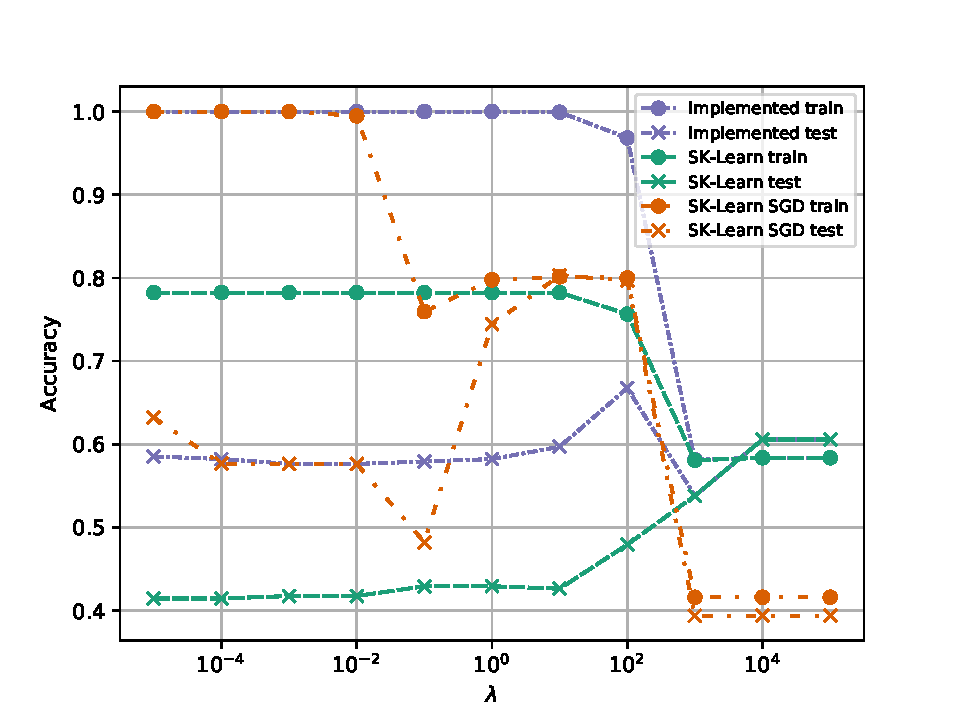
\includegraphics[scale=1.0]{../fig/logistic_accuracy_sklearn_comparison.pdf}
    \caption{The accuracy for our implementation of logistic regression versus that of SciKit learn.}
    \label{fig:logreg-accuracy-sklearn-comparison}
\end{figure}

\subsubsection{Classification through neural networks}
For classifying the states through a neural network, we looked at several different hyper parameters. All runs were made using $N_{samples}=10000$ except stated other wise. The training percent was 0.5. We start by comparing two different cost functions and their layer outputs,
\begin{itemize}
    \item Cross entropy with softmax layer output\eqref{eq:ce-mlp-cost}
    \item MSE with sigmoidal layer output.\eqref{eq:mse-mlp-cost}
\end{itemize}
These cost functions following behavior for epochs seen in following figure \ref{fig:mlp-cost-function-comparison},
\begin{figure}[H]
    \centering
    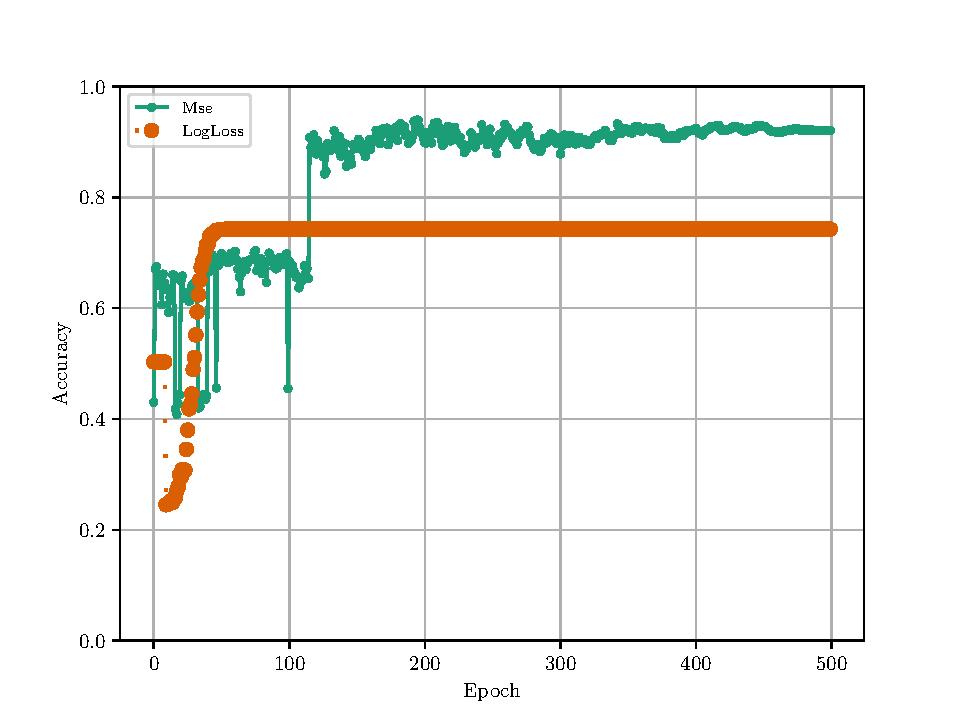
\includegraphics[scale=1.0]{../fig/mlp_epoch_cost_functions.pdf}
    \caption{A comparison in accuracy scores between the MSE and (CE) Cross Entropy loss functions over 500 epochs. The output layer for MSE is sigmoidal, the output layer for CE is softmax. The learning parameter was $\eta=0.001$ and we used the inverse learning rate\eqref{eq:inverse-eta}.}
    \label{fig:mlp-cost-function-comparison}
\end{figure}

We then wish to to investigate the effects of having different initial weights. Given the initial weights \textit{large} and \textit{default} as listed in section \ref{sec:nn-weights}, we get the results as seen in figure \ref{fig:mlp-epoch-init-weights},
\begin{figure}[H]
    \centering
    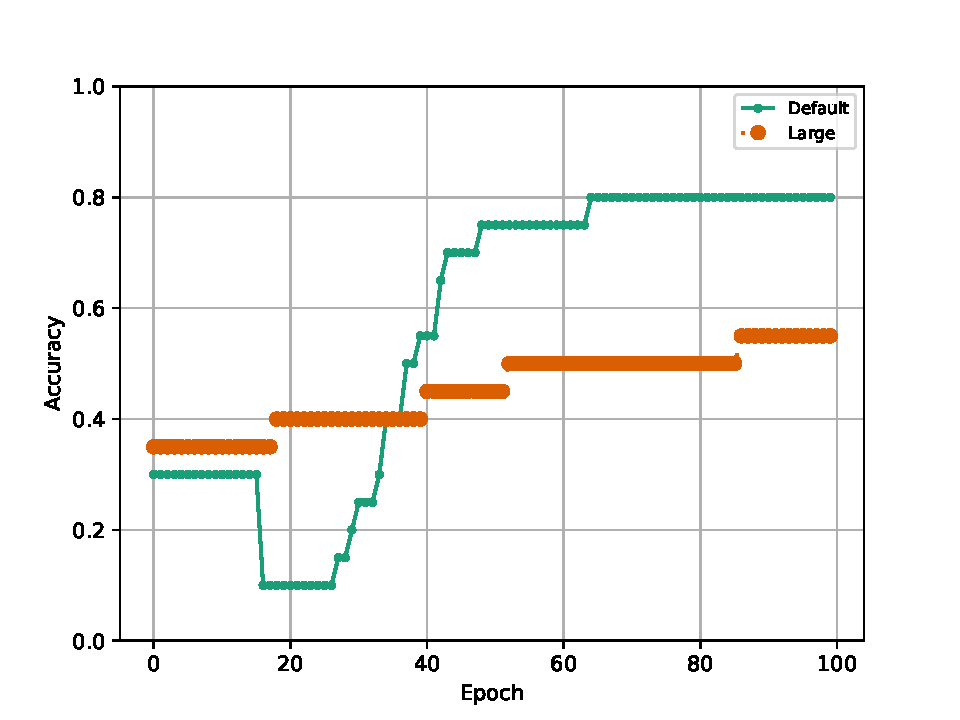
\includegraphics[scale=1.0]{../fig/mlp_epoch_weight_inits.pdf}
    \caption{A comparison in accuracy scores between the initial weights \textit{large} and \textit{default} as listed in section \ref{sec:nn-weights}. The run was for 500 epochs. The cost function was set to cross entropy and had softmax output activation. The learning parameter was $\eta=0.001$ and we used the inverse learning rate\eqref{eq:inverse-eta}.}
    \label{fig:mlp-epoch-init-weights}
\end{figure}

An investigation into different layer activations\ref{sec:layer-acts} was performed for both the MSE- and the CE-cost function. The results from MSE can be seen in figure 
\begin{figure}[H]
    \centering
    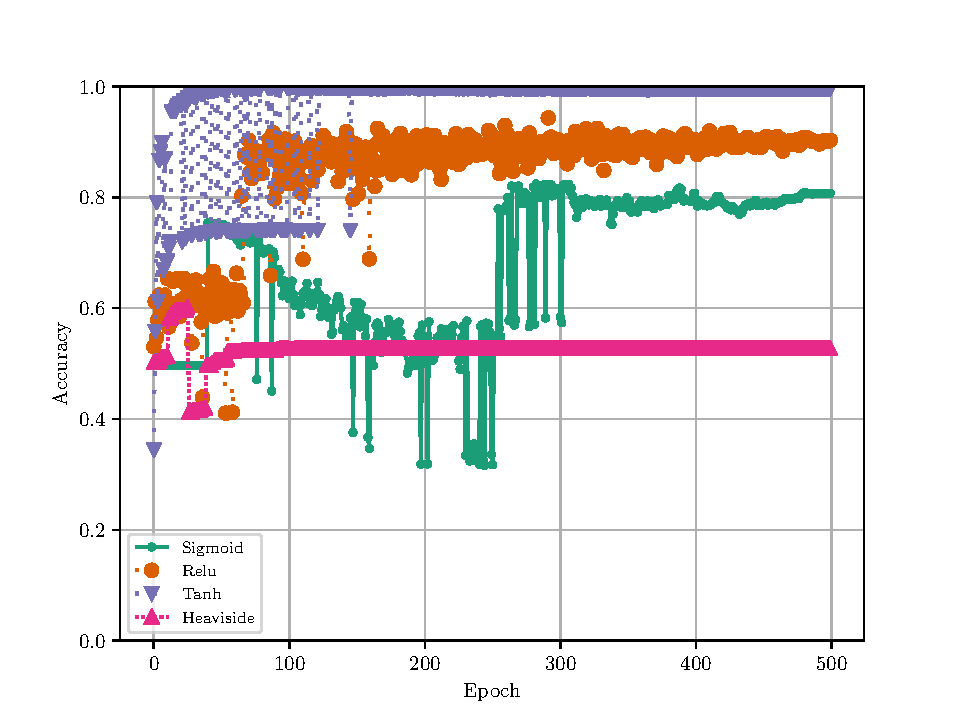
\includegraphics[scale=1.0]{../fig/mlp_epoch_activations_mse.pdf}
    \caption{A comparison in accuracy scores between the hidden layer activation functions(see section \ref{sec:layer-acts}) for MSE as cost function. The run was for 500 epochs. The learning parameter was $\eta=0.001$ and we used the inverse learning rate\eqref{eq:inverse-eta}.}
    \label{fig:mlp-epoch-activations-mse}
\end{figure}
\begin{figure}[H]
    \centering
    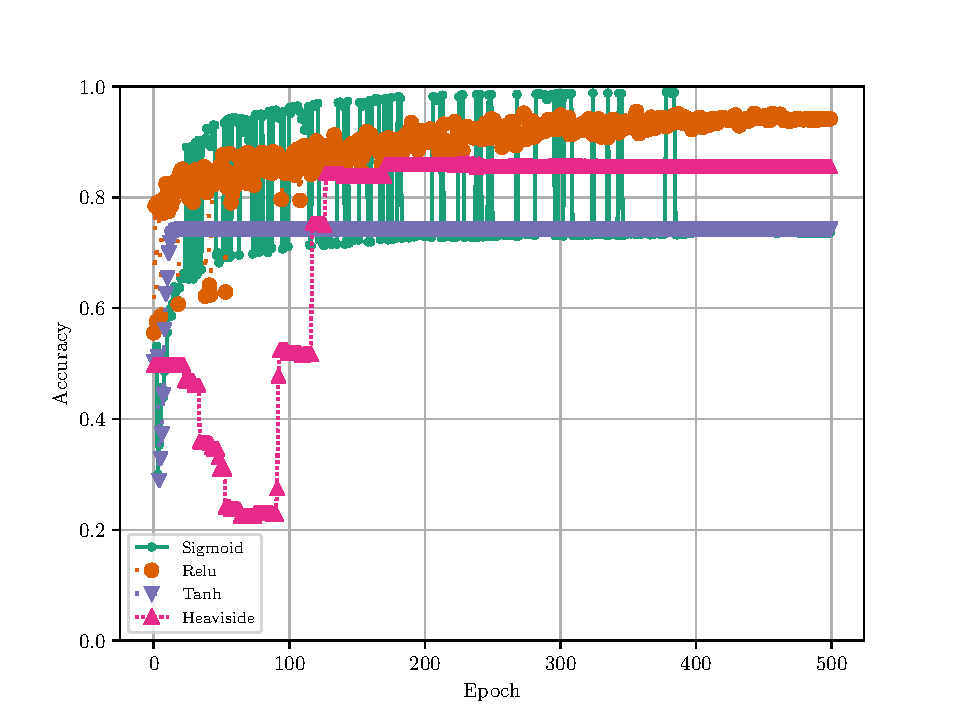
\includegraphics[scale=1.0]{../fig/mlp_epoch_activations_log_loss.pdf}
    \caption{A comparison in accuracy scores between the hidden layer activation functions(see section \ref{sec:layer-acts}) for cross entropy as cost function. The run was for 500 epochs. The learning parameter was $\eta=0.001$ and we used the inverse learning rate\eqref{eq:inverse-eta}.}
    \label{fig:mlp-epoch-activations-log-loss}
\end{figure}

We then move on to an investigation for different L$^2$ regularization strengths $\lambda$ versus different constant learning rates $\eta$. A run with 500 epochs, cross entropy and sigmoidal hidden layer activation can be seen in figure \ref{fig:mlp-eta-lambda},
\begin{figure}[H]
    \centering
    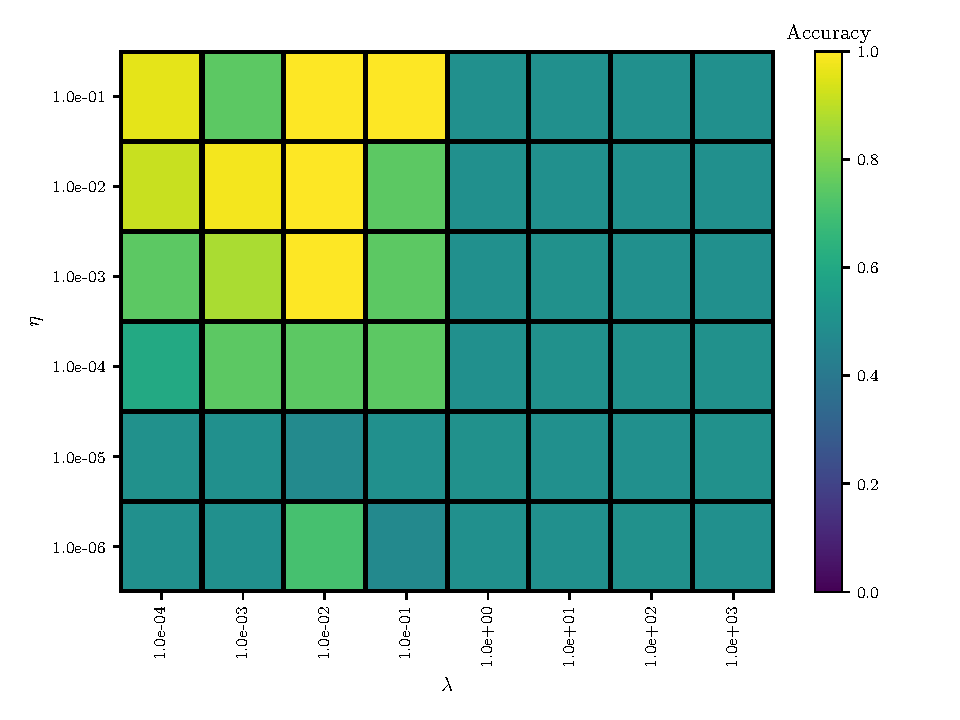
\includegraphics[scale=1.0]{../fig/mlp_lambda_eta.pdf}
    \caption{The accuracy as function of the L$^2$ regularization parameter $\lambda$ and constant training rate $\eta$. The run was for 500 epochs and with cross entropy as cost function, softmax output and sigmoidal hidden layer activation. The hidden layer was 10 neurons large.}
    \label{fig:mlp-eta-lambda}
\end{figure}

A comparison of the accuracy score\eqref{eq:mlp-accuracy} as a function of L$^2$ regularization parameter and hidden layer size(the neurons) can be viewed in figure \ref{fig:mlp-lambda-neurons}.
\begin{figure}[H]
    \centering
    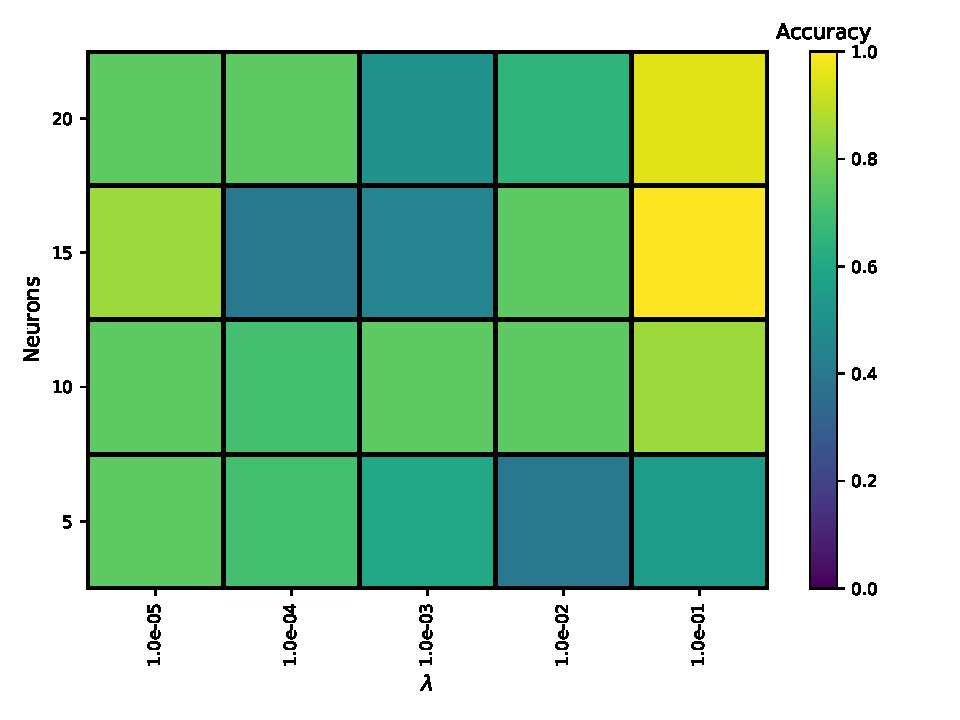
\includegraphics[scale=1.0]{../fig/mlp_lambda_neurons.pdf}
    \caption{The accuracy score as function of the L$^2$ regularization parameter $\lambda$ and the number of neurons. The run was for 500 epochs and with cross entropy as cost function, softmax output and sigmoidal hidden layer activation.}
    \label{fig:mlp-lambda-neurons}
\end{figure}

The accuracy score\eqref{eq:mlp-accuracy} as a function of the hidden layer size(the neurons) and the training data size as percentage of of a $N_\mathrm{samples}=10000$ training data, can be viewed in figure \ref{fig:mlp-neurons-ts}.
\begin{figure}[H]
    \centering
    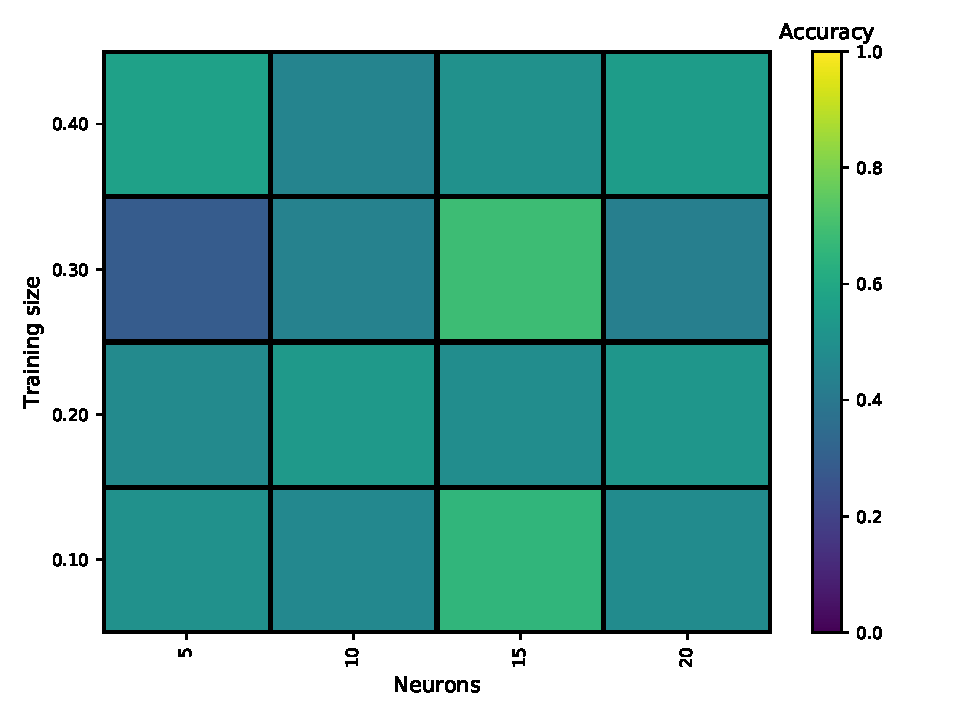
\includegraphics[scale=1.0]{../fig/mlp_neurons_training_size.pdf}
    \caption{The accuracy score as function of the number of neurons and the training data size percentage of $N_\mathrm{samples}=10000$. The run was for 500 epochs and with cross entropy as cost function, softmax output and sigmoidal hidden layer activation.}
    \label{fig:mlp-neurons-ts}
\end{figure}

The accuracy score\eqref{eq:mlp-accuracy} as a function of the hidden layer size(the neurons) and the learning rate $\eta$, can be viewed in figure \ref{fig:mlp-neurons-ts}.
\begin{figure}[H]
    \centering
    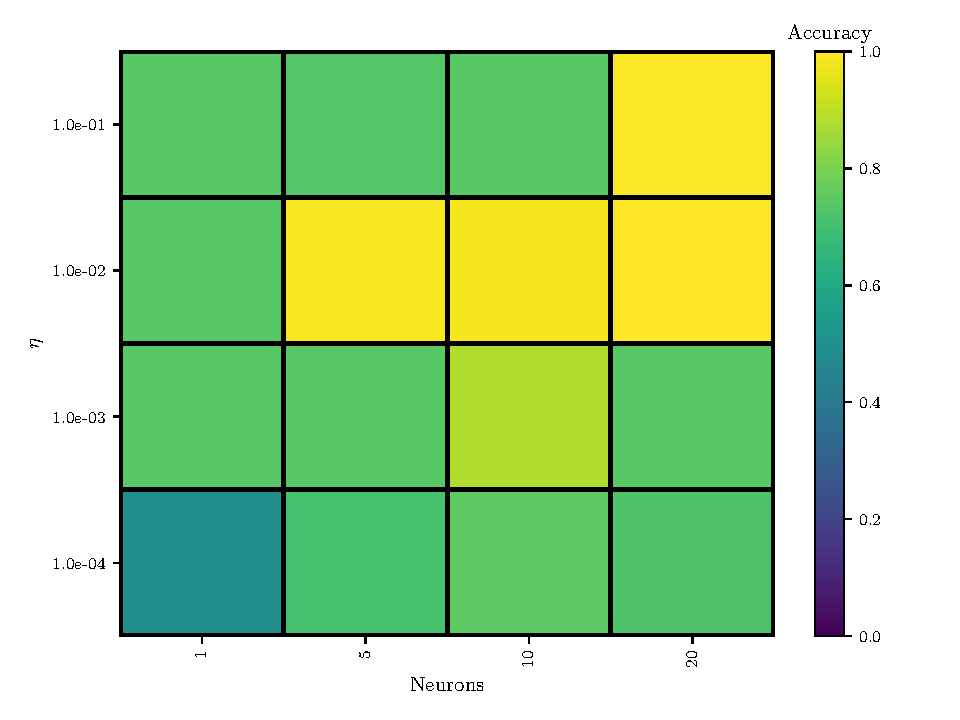
\includegraphics[scale=1.0]{../fig/mlp_neurons_eta.pdf}
    \caption{The accuracy score as function of the number of neurons and the learning rate $\eta$. The run was for 500 epochs and with cross entropy as cost function, softmax output and sigmoidal hidden layer activation.}
    \label{fig:mlp-neurons-eta}
\end{figure}

The accuracy score\eqref{eq:mlp-accuracy} as a function of L$^2$ regularization strength $\lambda$ and the mini batch size in the SGD\ref{alg:sgd}, can be viewed in figure \ref{fig:mlp-lambda-mb}.
\begin{figure}[H]
    \centering
    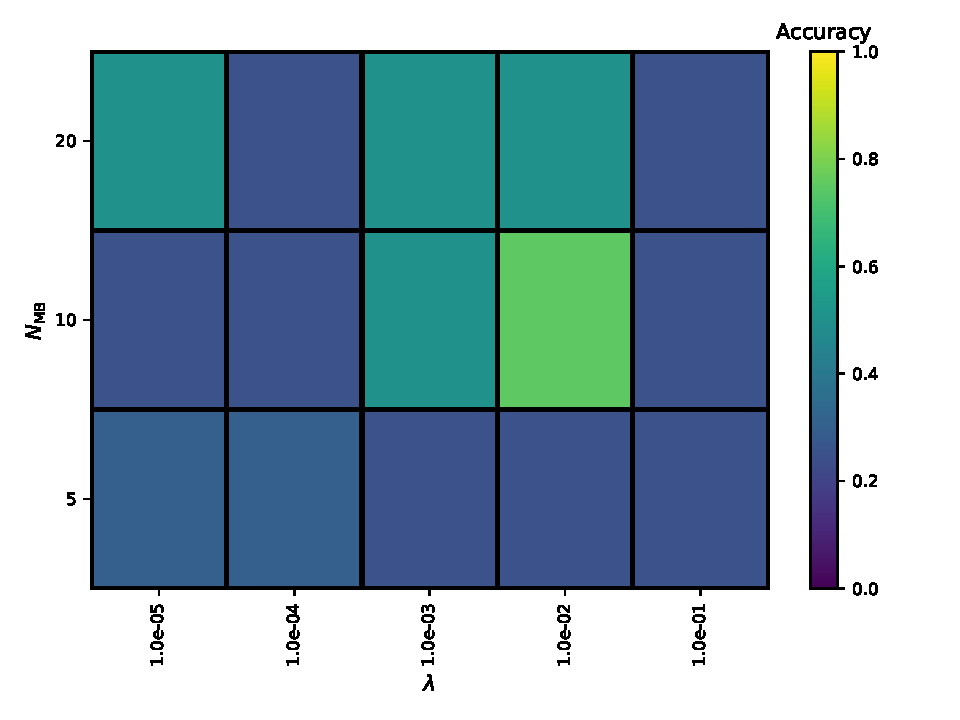
\includegraphics[scale=1.0]{../fig/mlp_lambda_mini_batch_size.pdf}
    \caption{The accuracy score as function of the  L$^2$ regularization strength $\lambda$ and the mini batch size in the SGD\ref{alg:sgd}. The run was for 500 epochs and with cross entropy as cost function, softmax output and sigmoidal hidden layer activation and the inverse learning rate \eqref{eq:inverse-eta}.}
    \label{fig:mlp-lambda-mb}
\end{figure}
